\chapter{Implementación}

\section{Algoritmos Relevantes}

    \subsubsection{Procesamiento Nodal}

        Un cliente en particular recibe un trabajo para realizar y lo procesa hasta su finalización permitiendo
        también la posibilidad de envío de mensajes y resultados al servidor en medio de la ejecución. En
        el algoritmo \ref{Alg-DRP} puede apreciarse mas detalladamente como el procesador recursivo opera para
        tal fin.\\

%     functorsList.push_back = deserialize(packet);
%
%     while(functors_list.have_elements())
%        {
%             current_functor = functors_list.pop_back()
%             children = []
%             current_functor.call(children, message);
%
%             if (!message.empty())
%                 if ( children.empty() )
%                     send_result(message)
%                 else
%                     send_message(message);
%
%             functors_list.concat(children);
%
%             if time_to_dispatch() then
%                 dispatch_children(functor_list)
%     }

    \renewcommand{\algorithmicrequire}{\textbf{Input:}}
    \renewcommand{\algorithmicensure}{\textbf{Output:}}

    \algsetup{indent=1cm,linenodelimiter=.}
    \begin{algorithm}[!ht]
        \caption{Procesamiento de un Functor. \texttt{do\_recursion}}\label{Alg-DRP}
        \begin{algorithmic}[1]
        \REQUIRE $Packet$
        \STATE $FunctorList \gets [deserialize(Packet)]$
        \STATE $\ $
        \WHILE{\NOT $FunctorList.is\_empty()$}
            \STATE $CurrentFunctor \gets FunctorList.pop\_back()$
            \STATE $CurrentChildren \gets [\ ]$
            \STATE $\ $
            \STATE $CurrentFunctor.call(CurrentChildren, Message, Result)$
            \STATE $\ $
            \IF {\NOT$Result.is\_empty()$}
                \STATE $send\_result(Result)$
            \ELSE
                \IF{\NOT $Message.is\_empty()$}
                    \STATE $send\_message(Message)$     
                \ENDIF
            \ENDIF
            \STATE $\ $
            \STATE $FunctorList.append(CurrentChildren)$
            \STATE $\ $
            \IF{$IsTimeToDispatch()$}
                \STATE $dispatch\_children(FunctorList)$
            \ENDIF
        \ENDWHILE

        \end{algorithmic}
    \end{algorithm}

    Básicamente el algoritmo mantiene una lista (al comienzo inicializada con el functor inicial) que tiene todos los functores
    sin procesar, hasta que esta lista no quede totalmente vacía se extrae el de más a la derecha y se lo reproduce.\\

        \begin{figure}[!ht]
            \begin{center}
                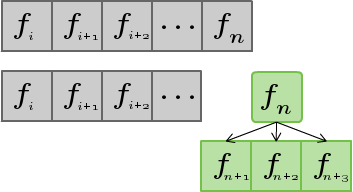
\includegraphics[scale=0.6]{images/DRP-Alg-1.png}
            \end{center}
            \caption{Lista de functores pendientes de ejecución}
        \end{figure}

    Esta reproducción implica por parte de la aplicación la responsabilidad de depositar en \textit{CurrentChildren} los functores
    resultantes de avanzar un paso en la recursión, un mensaje si lo desea y el resultado de la operacion en caso de que el functor llegue
    a un caso base.

    Luego, estos nuevos \textit{``functores hijos''} son agregados a la lista en la parte de atrás. Si los comparamos
    por \textit{``pasos inductivos restantes''} la lista queda ordenada de mayor a menor.\\

        \begin{figure}[!ht]
            \begin{center}
                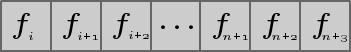
\includegraphics[scale=0.6]{images/DRP-Alg-2.png}
            \end{center}
            \caption{Lista de functores ordenada}
        \end{figure}

    Por este orden es que a la hora de delegar trabajo a otro cliente se opta por sacar los functores más a la
    izquierda, aquí se pregunta por la disponibilidad de clientes ociosos y el servidor le dirá de cuantos functores se
    puede desligar. Supongamos que el servidor luego de la petición haya reservado dos clientes, el nodo corriente se
    los enviará y seguirá su ejecución con el resto.\\

        \begin{figure}[!ht]
            \begin{center}
                
\includegraphics[scale=0.6]{images/DRP-Alg-3.png}
            \end{center}
            \caption{Criterio de redistribución}
        \end{figure}

    Cabe aclarar que la complejidad temporal de este algoritmo depende estrictamente del problema particular que se
    corra sobre \rc{}. Sea $f$ la función que representa el comportamiento del algoritmo \ref{Alg-DRP}, $c$ la cantidad máxima de hijos
reproducidos por paso de recursión, $h$ la profundidad máxima del árbol
    de recursión resultante de correr el programa para una entrada particular y $g$ el orden de complejidad de la
    reproducción del functor podemos decir que:

    \begin{table}[ht]
        \begin{center}
        $$T(f(c,h)) = O(\displaystyle\sum\limits_{i=1}^{h} {c^i})*O(g)$$
        \end{center}
    \end{table}

\section{Métricas de Código}

Para analizar el código estáticamente se usaron herramientas como CLOC\footnote{http://cloc.sourceforge.net/} (Count Lines of Code) y
CCCC\footnote{http://cccc.sourceforge.net/} (\textbf{\textit{C}} and \cpp{} Code Counter). En esta sección se describen métricas de
código generales obtenidas por ambas herramientas y se analizan los resultados obtenidos.

\subsection{Métricas de \rc}
\label{recabs_metrics}

\rc{} esta constituido por 23 archivos con un total de 2394 líneas de texto a la fecha de publicación de este documento. La tabla
\ref{cloc_recabs} resume los resultados obtenidos después de correr la herramienta CLOC sobre los archivos fuentes de \rc.

\begin{table}[!htf]
    \begin{center}
    \begin{tabular}{|l|r|r|r|r|c|}
    \hline
    \multicolumn{2}{|c|}{Files} & \multicolumn{3}{|c|}{Line Types} & \hspace{0.2cm}\% \\
    \hline
    \textbf{Type} & \textbf{Count} & \textbf{Blank} & \textbf{Comment} & \textbf{Source} & \small{\textbf{\#Comms./Tot.}}\\
    \hline
    \texttt{C++ source} & 7   &    102  &     301   &    381 & 44.13 \\
    \hline
    \texttt{C++ header} & 16   &    231  &    1010   &    369 &  73.24 \\
    \hline
    \textbf{Total}      &  23  &     333 &     1311  &    750 & 63.6 \\
    \hline
    \end{tabular}
    \caption{Resultados de CLOC para la capa \rc}
    \label{cloc_recabs}
    \end{center}
\end{table}

Los resultados revelan que \rc{} no es un proyecto de gran tamaño. Sin embargo, estas medidas no reflejan su complejidad.

Dijkstra escribió un ensayo muy interesante\cite{ewd1036} donde reflejaba por qué las empresas no deberían considerar las Líneas de Código
como una medida exacta de la productividad del software. Medir la ``productividad de un programador'' en términos del ``número de líneas de
código que produce por mes'' fomenta la escritura de código insípido.

Por otro lado, a mayor número de líneas de código mayor es la complejidad de un producto de software, pero sólo en el sentido de que es
más dificultoso de mantener y comprender, no tiene relación directa con la funcionalidad que éste provee.

Continuando con el análisis sobre los resultados de CLOC, otro dato interesante es la cantidad de líneas de comentarios en el proyecto y su
porcentaje con respecto al total de líneas de código efectivas del proyecto. La siguiente fórmula describe la relación comentarios/código y
la misma fue usada para calcular la última columna de la tabla \ref{cloc_recabs}:

$$\frac{\#comment\_lines}{\#comment\_lines + \#code\_lines}$$

Este valor ronda el 0.63, lo que significa que hay más líneas de comentarios que líneas de código. Este porcentaje de líneas de comentarios
se debe, en mayor medida, a que por cada archivo (por más pequeño que sea) se incluye una cabecera (``header'') definiendo ciertos detalles
del archivo: como sus autores, fecha de creación y la licencia por cual se rige.

Para aún justificar más la alta cantidad de comentarios en \rc, todo componente de software (clases, estructuras, funciones, atributos,
etc.) tiene una descripción detallada a ser interpretada por \textit{Doxygen} (el cuál incluye perfiles de funciones) para la generación de
documentación automática. El ejemplo \ref{recabs_comment} muestra la notación utilizada para Doxygen exhibiendo además el porqué de la alta
tasa de comentarios.

\begin{table}[!h]
    \lstset{language=C++}
    \begin{lstlisting}[frame=single]
/**
 * How many functors are sent to the server ?
 * Should be implemented as a way to distribute work.
 * This function should never return more than n_children-1 and less
 * than 0. In other words, should return a integer k, such that:
 *                     0 <= k < n_children
 *
 * @param n_children : the number of children in the current step.
 * @param depth      : current depth of the recursion tree.
 * @returns the number of children to redistribute.
 */
virtual uint how_much_distribute(uint n_children, uint depth) const = 0;
    \end{lstlisting}
    \centering \caption{Comentario de una función en \rc.}
    \label{recabs_comment}
\end{table}

Por otro lado, el uso extensivo de librerías permitió la minimización de código, el ejemplo exhibido en \ref{using_fud_lib} es un buen
ejemplo para mostrar que en 5 líneas de código, este método inicia el servidor, creando un thread para escuchar paquetes entrantes y varios
otros hilos de ejecución para crear unidades de trabajo y enviarlos a clientes conectados por toda la red, tolerando cortes de
comunicación abruptos y demás funciones que permiten el buen desempeño de distribución de tareas, en resumen, el ahorro de muchas líneas de
código. La librería \fud{} fue la más utilizada en el desarrollo de este proyecto, y en menor medida se utilizó la librería
\textit{\textbf{MiLi}}.

\begin{table}[!h]
    \lstset{language=C++}
    \begin{lstlisting}[frame=single]
void FuDRManager::start()
{
    /* Get the initial packet. */
    Packet initial_packet;
    _server_app.get_initial_packet(initial_packet);

    /* Push initial packet in the stack. */
    push_child(initial_packet);
  
    /* Run the unique DistributableJob. */
    this->run();
    this->wait_completion();    
}
    \end{lstlisting}
    \centering \caption{Ejemplo de uso de la librería \fud}
    \label{using_fud_lib}
\end{table}

En el apéndice \ref{recabs_metrics_report} se muestra un reporte completo sobre las métricas de código de \rc{} generado con la herramienta
CCCC. Incluye muchas métricas de diseño Orientado a Objetos y todo tipo de información relevante en cuanto a código. Un análisis exhaustivo
de los resultados de estas métricas está fuera del alcance de este trabajo. No obstante, el informe proporciona una visión cuidadosa de la
estructura de la librería.

\subsubsection{Cobertura de Código para \rc}
\label{cobertura_recabs}

Es una medida cuantitativa utilizada en pruebas de software que describe el grado de código fuente \textit{testeado}, lo cuál funciona como
una medida indirecta de calidad. En la tabla \ref{recabs_gcov} se muestra la cobertura de código de los archivos de mayor relevancia en
\rc. La cobertura fue hecha corriendo la aplicación \textit{Binary Search} que será introducida en la siguiente sección.

Analizando los resultados de la cobertura de sentencia realizada, más específicamente las líneas no visitadas, sabemos que:
\begin{itemize}
    \item   En el módulo \texttt{DistributionPolicy} las líneas no ejecutadas se deben a que se usa sólo una política de distribución, por
            lo que los demás algoritmos de distribución no son utilizados.
    \item   En el resto de los archivos, las líneas no visitadas corresponden al manejo de errores.
\end{itemize}

La prueba fue realizada con la herramienta \textbf{gcov}\footnote{http://gcc.gnu.org/onlinedocs/gcc/Gcov.html}, corriendo la misma
aplicación 20 veces, variando la cantidad de clientes conectados e interrumpiendo algunos de ellos en su ejecución. En estas pruebas, el
sistema funcionó como se esperaba.

\begin{table}[!htf]
    \begin{center}
    \begin{tabular}{|l|r|r|c|}
        \hline
        & \multicolumn{2}{|c|}{Líneas de código} & Porcentaje \\
        \hline
        \textbf{Archivo} & \textbf{Total} & \textbf{Ejecutado} & \hspace{0.2cm}\textbf{\%} \\
        \hline
        \scriptsize{distributable\_recursive\_processor.cpp} & 91 & 78 & 85.7 \\
        \hline 
        \scriptsize{distribution\_policy.cpp} & 27 & 17 & 62.9 \\
        \hline 
        \scriptsize{by\_size\_result\_sender.cpp} & 18 & 18 & 100 \\
        \hline 
        \scriptsize{fud\_rprocessor.cpp} & 18 & 18 & 100 \\
        \hline 
        \scriptsize{recursion\_manager.cpp} & 37 & 34 & 91.8 \\
        \hline 
        \scriptsize{fud\_rmanager.cpp} & 36 & 35 & 97.2 \\
        \hline 
        \textbf{Total} & 227 & 200 & 88.1 \\
        \hline
    \end{tabular}
    \caption{Resultados de cobertura para los principales archivos de \rc}
    \label{recabs_gcov}
    \end{center}
\end{table}
